\documentclass[a4paper]{article}

\renewcommand{\contentsname}{Obsah} %rename ToC to Obsah
\renewcommand{\refname}{Literatura} %rename Bibliography to Literatura

%--------packages
\usepackage{graphicx} % images
\graphicspath{figures/}
\usepackage[hidelinks]{hyperref} %clickable images
\usepackage{amsmath}
\usepackage{amsfonts}
\usepackage{mathtools}

\title{Barevné polarizační zobrazování pro bioaplikace \\rešerše}
\author{Prokop Beneš}
\date{Prosinec 2024}

\numberwithin{equation}{section}

\begin{document}
	\maketitle
	\newpage

	\tableofcontents
	\newpage

    \section{Úvod}
    Barevné polarizační zobrazování představuje inovativní přístup k analýze optických vlastností materiálů,
    který se stále více prosazuje v mnoha oborech a to i v medicínských tak i biologických aplikacích.
    Využití polarizace světla umožňuje získávat informace o strukturálních a povrchových vlastnostech vzorků,
    které jsou běžnými metodami prakticky nedostupné. \cite{photonics}
    \\Tato práce si klade za cíl teoreticky zpracovat problematiku barevného polarizačního zobrazování z
    pohledu fyziky a prozkoumat jeho možnosti v biologických aplikacích, zejména při studiu rostlinných vzorků.
    V této práci bude využita polarizační kamera BFS-U3-51S5PC-C s integrovaným senzorem Sony IMX250MYR,
    přičemž se zaměříme na její schopnost snímat a kombinovat polarizační a barevná obrazová data. \cite{flir}\cite{teledyne}\cite{senzor}
	\newpage
        
	\section{Polarizace}
    Elektromagnetické vlny mají velmi široký spektrální interval. My budeme uvažovat elektromagnetické vlnění
    pro nás viditelné. Tento interval elektromagnetického vlnění se nachází v intervalu přibližně 380 - 720nm.
    O elektromagnetickém vlnění v tomto intervalu budeme mluvit jako o světle. \cite{maly}
    \\Elektromagnetická postupná vlna je vlna příčná, což znamená, že elektrické a magnetické pole jsou kolmé
    na směr šíření. To znamená, že existuje dva nezávislé směry pro vektory těchto polí, mluvíme o dvou
    nezávislých My se zaměříme na popis elektrické složky vlny $\vec{E}$, protože vektor magnetické složky
    $\vec{B}$ je určena vztahem $\vec{B}= \frac{1}{v}\vec{s}\times\vec{E}$, kde $\vec{s}$ je vektor udávající
    směr šíření. Když zvolíme souřadný systém tak, že směr šíření je $\vec{s}=z$. Pak můžeme jako bázi příčné
    roviny, ve které se nachází $\vec{E}$, použít osy $x$ a $y$. Obecný vektor elektrického pole pak lze
    rozložit na složky směřující podél souřadných os.


    %dooznačit všechny proměnné!!!!!!!!!!!!!!!!!!!!!!!!!!!!!
    \begin{equation} \label{eq:1}
        \vec{E} = E_x\vec{x} + E_y\vec{y}
    \end{equation}
    Pokud budeme uvažovat harmonické postupné vlny, můžeme díky principu superpozice zvolit vlnu s různou
    amplitudou a s různým fázovým posunem:
    \begin{equation} \label{eq:2}
        \vec{E}(\vec{r},t) = E_{x0} e^{i(\omega t - kz + \varphi_1)} \vec{x} + 
                             E_{y0} e^{i(\omega t - kz + \varphi_2)} \vec{y}
    \end{equation}
    Fázový rozdíl těchto dvou složek můžeme vyjádřit jako 
    \begin{equation} \label{eq:3}
        \delta \varphi = (\omega t -kz + \varphi_1) - (\omega t -kz + \varphi_2) = \varphi_1 - \varphi_2
    \end{equation}
    ten nezávisí ani na čase ani na poloze v prostoru. Zvolíme si libovolné místo v prostoru jako
    $z = z_0$, můžeme sledovat časový průběh elektrického pole $\vec{E}(t) = \vec{E}(z_0,t)$
    \begin{equation} \label{eq:4}
        \vec{E}(t) = E_{x0} \vec{x} e^{i(\omega t + \varphi_1')} + E_{y0} \vec{y} e^{i(\omega t + \varphi_2')}
    \end{equation}
    kde $\varphi_i' = \varphi - kz_0$. Znovu tedy platí to samé pro rozdíl fází
    \begin{equation} \label{eq:5}
        \delta \varphi = \varphi_1 - \varphi_2 = \varphi_1' - \varphi_2' = (\varphi_1 - kz_0) - (\varphi_2 - kz_0)
    \end{equation}
    Z toho tedy vyplývá, že pro fázový rozdíl není důležité, ve kterém místě budeme průběh elektrického pole
    sledovat. Není třeba se zaobírat konrétními hodnotami fází, rozlišujeme pouze jejich rozdíl $\delta \varphi$.
    Reálná část rovnice (\ref{eq:4}) má tvar:
    \begin{equation} \label{eq:6}
        \vec{E}(t) = E_{x0}\vec{x}\cos(\omega t + \varphi_1) + E_{y0}\vec{y}\cos(\omega t + \varphi_2)
    \end{equation}
    je parametrickou rovnicí elipsy. Vektor elektrického pole $\vec{E}$ tedy v daném místě opisuje křivku,
    která má tvar elipsy. Tato elektromagnetická vlna je tedy elipticky polarizovaná. 
    \\Vlny tvaru (\ref{eq:4}), můžeme psát pomocí komplexního vektoru o dvou složkách $\hat{\vec{E}} \in \mathbb{C}^2$, 
    \begin{equation}
        \vec{E}(z,t) = \big(E_{x0} e^{i\varphi_1} \vec{x} + E_{y0} e^{i\varphi_2} \vec{y} \big)  e^{i(\omega t - kz)} = \hat{\vec{E}} e^{i(\omega t-kz)}
    \end{equation}
    \begin{equation}
        \hat{\vec{E}} = \begin{pmatrix} \hat{E}_1 \\ \hat{E}_2 \end{pmatrix} = \begin{pmatrix} E_{x0} \, e^{i \varphi_1} \\ E_{y0} \, e^{i \varphi_2} \end{pmatrix}	 \in \mathbb{C}^2
    \end{equation}
    \\Jeden pro nás velmi důležitý speciální případ je vlna, která je lineárně polarizovaná. Ta nastává,
    pokud vektor elektrické intenzity $\vec{E}$ kmitá jednom daném směru. 
    \\Tento případ nastává pro fázový posun $\delta \varphi \in \{0,\pi\}$, což pak můžeme zapsat jako
    \begin{equation} \label{eq:7}
        \vec{E} = E_0 \vec{n} e^{i(\omega t + \varphi]}
    \end{equation}
    neboli 
    \begin{equation} 
        \hat{\vec{E}} = E_0 \, \vec{n} \, e^{i\varphi} = E_0 \begin{pmatrix} \cos \theta \\ \sin \theta \end{pmatrix} e^{i\varphi}
    \end{equation}
    kde jednotkový vektor $\vec{n} = (n_x,n_y) = (\cos \theta, \sin \theta)$ znázorňuje směr kmitání
    elektrického pole $\vec{E}(t)$ v rovině $xy$ a úhel $\theta$ značí odklon tohoto vektoru od osy $x$. \cite{schmidt}
    \\Jedním z nejobvyklejších způsobů kde se v životě potkáme s polarizovaným světlem je bězná polarizace odrazem. 
    Tento proces vychází ze Snellova zákona následujícím způsobem: 
    \begin{equation}
        n_1 \sin \theta_i = n_2 \sin \theta_t
    \end{equation}
    je Snellův zákon a $n_1$ a $n_2$ značí index lomu daného prostředí v kterém se světlo šíří. 
    $\theta_i$ je úhel dopadu, $\theta_t$ je úhel lomu. Úhlu pod kterým musí světlo dopadnout aby bylo lineárně
    polarizováno se říká úhel Brewsterův. 
    \begin{figure}[h]
        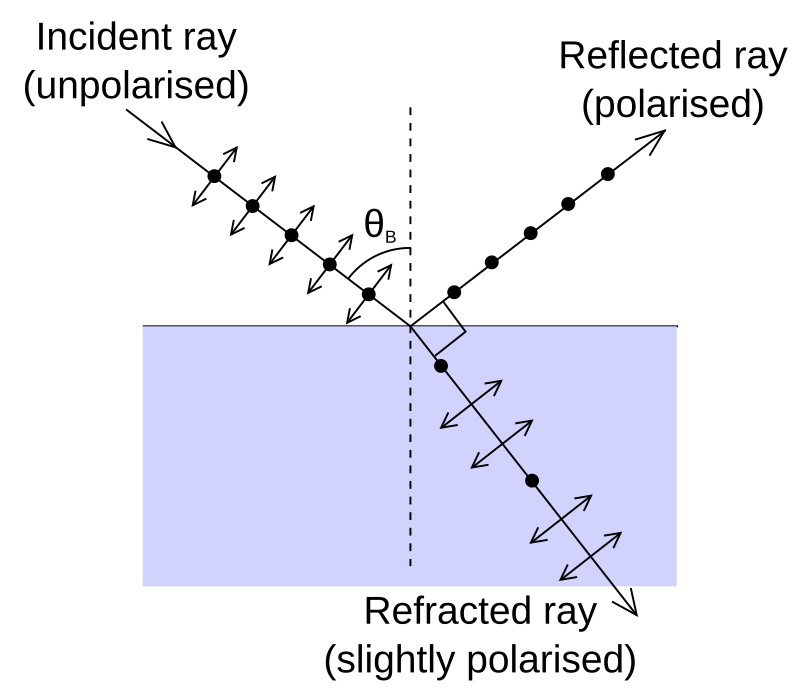
\includegraphics[width=7cm]{figures/Brewster.png}
        \centering
    \end{figure}
    \\Pro něj platí že $\theta_i + \theta_t = 90^{\circ}$, tedy, že úhel
    dopadajícího, tedy i odraženého světla musí svírat se světlem lomeným úhel devadesáti stupňů. Tedy 
    $\theta_t = 90^{\circ} - \theta_i$ dosadíme do Snellova zákona. 
    \begin{equation}
        \!
        \begin{aligned}
            n_1 \sin \theta_i &= n_2 \sin (90^{\circ} - \theta_i) \\
            n_1 \sin \theta_i &= n_2 \cos \theta_i
        \end{aligned}
    \end{equation} 
    což nám po úpravě dá 
    \begin{equation}
        \frac{n_2}{n_1} = \frac{\sin \theta_i}{\cos \theta_i}
    \end{equation}
    neboli
    \begin{equation}
        \tan \theta_i = \frac{n_2}{n_1}
    \end{equation}
    Kde námi požadovaný Brewsterův úhel dostaneme jako
    \begin{equation}
        \theta_B = \arctan \frac{n_2}{n_1}
    \end{equation}
    Nepolarizované světlo dopadjící pod tímto úhlem se od rozhraní odráží pouze se složkou kolmou k rovině
    rozhraní. \cite{hecht} 
    \\Takto lineárně polarizované světlo pro nás bude v následujícím textu velmi důležité. Na princip lineárně
    polarizovaného světla totiž stojí princip naší barevné polarizované kamery BFS-U3-51S5PC-C

    \newpage
	\section{Aplikace Polarizace}
	Senzor kamery s kterou pracujeme má na svém senzoru mikrostrukturu, která se chová jako polarizátor
    přicházejícího světla, jelikož je jeho rozměr dostatečně malý na to, aby jím prošla jen určitá složka světla
    v daném úhlu podle úhlu samotného polarizátoru. Senzor samotný má každý pixel sestaven ze čtyř podpixelů
    kde každý z nich má přes sebe jiný úhel polarizátoru a to $90^{\circ}, 45^{\circ}, 135^{\circ}, 0^{\circ}$
    podle směru hodinových ručiček začínaje vlevo v rohu.
    \begin{figure}[h]
        \includegraphics[width=8cm]{figures/senzor.jpg}
        \centering
    \end{figure}

	\newpage
	\section{Získání dat z polarizační kamery}

    \newpage
    \addcontentsline{toc}{section}{Literatura}
    \begin{thebibliography}{99}
        \bibitem{hecht} Hecht E., \textit{Optics}, 4th Ed, Pearson, 2002
        \bibitem{maly} Malý P., \textit{Optika}, Nakladatelství Karolinum, 2008
        \bibitem{schmidt} Schmidt J., \textit{Vlnění, optika a atomová fyzika}, \url{https://physics.fjfi.cvut.cz/~schmijos/voaf/skriptaVOAF.pdf}
        \bibitem{flir} \url{https://www.flir.eu/globalassets/support/iis/knowledge-base/getting-started-with-bfs-polarized-cameras.pdf}
        \bibitem{teledyne} \url{https://www.teledynevisionsolutions.com/learn/learning-center/machine-vision/imaging-reflective-surfaces-sonys-first-polarized-sensor/}
        \bibitem{photonics} \url{https://www.photonics.com/Articles/Polarization-Based_Imaging_Basics_and_Benefits/a60734}
        \bibitem{senzor} \url{https://www.sony-semicon.com/files/62/flyer_industry/IMX250_264_253MZR_MYR_Flyer_en.pdf}
    \end{thebibliography}
\end{document}